\documentclass[12pt,a4paper]{beamer}
%\usepackage[utf8x]{inputenc}
%\usepackage{ucs}
\usepackage{amsmath}
\usepackage{amsfonts}
\usepackage{amssymb}
\usepackage{graphicx}
\usepackage{wrapfig}
\usepackage{verbatim}

\author{Robin Ellerkmann, Sven Reber}
\title{Konflikthandhabung\\Theorie und Praxis}

\begin{document}
\maketitle

\begin{frame}
	\frametitle{Inhalt}
	
	\begin{itemize}
		\item Aufgabenstellung
		\item Fehlerfindung
		\begin{itemize}
			\item Verfahren 1: Nachbarwerte
			\item Verfahren 2: Quadratischer Fehler
			\item Verfahren 3: Einfach
		\end{itemize}
		\item Programmvorf\"uhrung
		\item Code-Rosinen
	\end{itemize}
\end{frame}

\begin{frame}
	\frametitle{Aufgabenstellung}
	
	\begin{figure}
		\begin{minipage}{0.45\linewidth}
			\begin{itemize}
				\item GUI
				\item Nifti laden/anzeigen
				\item DTI-Volumen durchlaufen
				\item Automatische Fehlererkennung
			\end{itemize}
		\end{minipage}
		%\begin{minipage}{0.45\linewidth}
		%	\includegraphics[width=1.0\linewidth]{programmfenster_v2.jpg} 
		%\end{minipage}
	\end{figure}

	%\begin{wrapfigure}{r}{3 cm}
	%	\centering
	%	\includegraphics[width=0.3\textwidth]{programmfenster.jpg} 
	%	\caption{XXX} % Bildunterschrift
	%\end{wrapfigure}
\end{frame}


\begin{frame}
	\frametitle{Fehlerfindung}
	\begin{itemize}
		\item Verfahren 1: Nachbarwerte
		\item Verfahren 2: Quadratischer Fehler
		\item Verfahren 3: Einfach
	\end{itemize}
\end{frame}

\begin{frame}
	\frametitle{Testdaten}
	\begin{figure}
		\centering
		%\includegraphics[width=0.6\textwidth]{fehlerhaft.jpeg} 
		\caption{Fehlerhafte .nii Daten} % Bildunterschrift
	\end{figure}
	frame(row, :) = randi(5, 1, 102);	
\end{frame}

\begin{frame}
	\frametitle{Fehlerfindung Verfahren 1: Nachbarwerte}
	\begin{itemize}
		\item Spaltenweise bzw. Zeilenwiese  durch die Layer der einzelnen Tensoren durchgehen
		\item betrachten nun jedes einzelne Voxel der Zeile bzw. Spalte
		\item errechnen aus den  korrespondierenden Voxel der Nachbartensoren  den gesch\"atzen Wert, f\"ur das zu qualifizierende Voxel
		\item ist der Wert des zu klassifizierden Voxels zu weit vom gesch\"atzten Wert entfernt, wird dieses Voxel als potentiell Fehlerhaft eingestuft
		\item sind zu viele Voxel in eine Spalte bzw. Zeile als potentiell Fehlerhaft eingestuft, wird diese Reihe als Fehlerhaft klassifiziert
	\end{itemize}
\end{frame}

\begin{frame}
	\frametitle{Fehlerfindung Verfahren 2: Quadratischer Fehler}

	\begin{itemize}
		\item berechne \textbf{quad. Fehler}  für ein Tensor-Bild mit
		\begin{itemize}
			\item einer \textit{Schicht}
			\item einer Zeile 
			\item zw. aktuellem und folgendem Tensor-Bild
		\end{itemize}
		\item bestimme \textbf{Standartabweichung} aller \textbf{quad. Fehler} einer \textit{Schicht}
		\item Differenz von vorheriger und nachfolgender Reihe sollte kleiner der Standartabweichung sein
	\end{itemize}
	
	\begin{align*}
		\text{qerror}(\text{row}) &- \text{qerror}(\text{row}-1)  > \text{std}(\text{frame}) \;\;\&\& ... \\
		\text{qerror}(\text{row}) &- \text{qerror}(\text{row}+1) > \text{std}(\text{frame})
	\end{align*}
\end{frame}

\begin{frame}
	\frametitle{Fehlerfindung Verfahren 3: Einfach}
	\begin{itemize}
		\item Normierung auf 255 Grauwerte
		\item Suche nach Zeilen, die nur 0 oder 1 enthalten
		\item ignoriere Zeile 1 und 102!
	\end{itemize}
\end{frame}

\begin{frame}
	\frametitle{Programmvorf\"uhrung}
	\begin{center}
		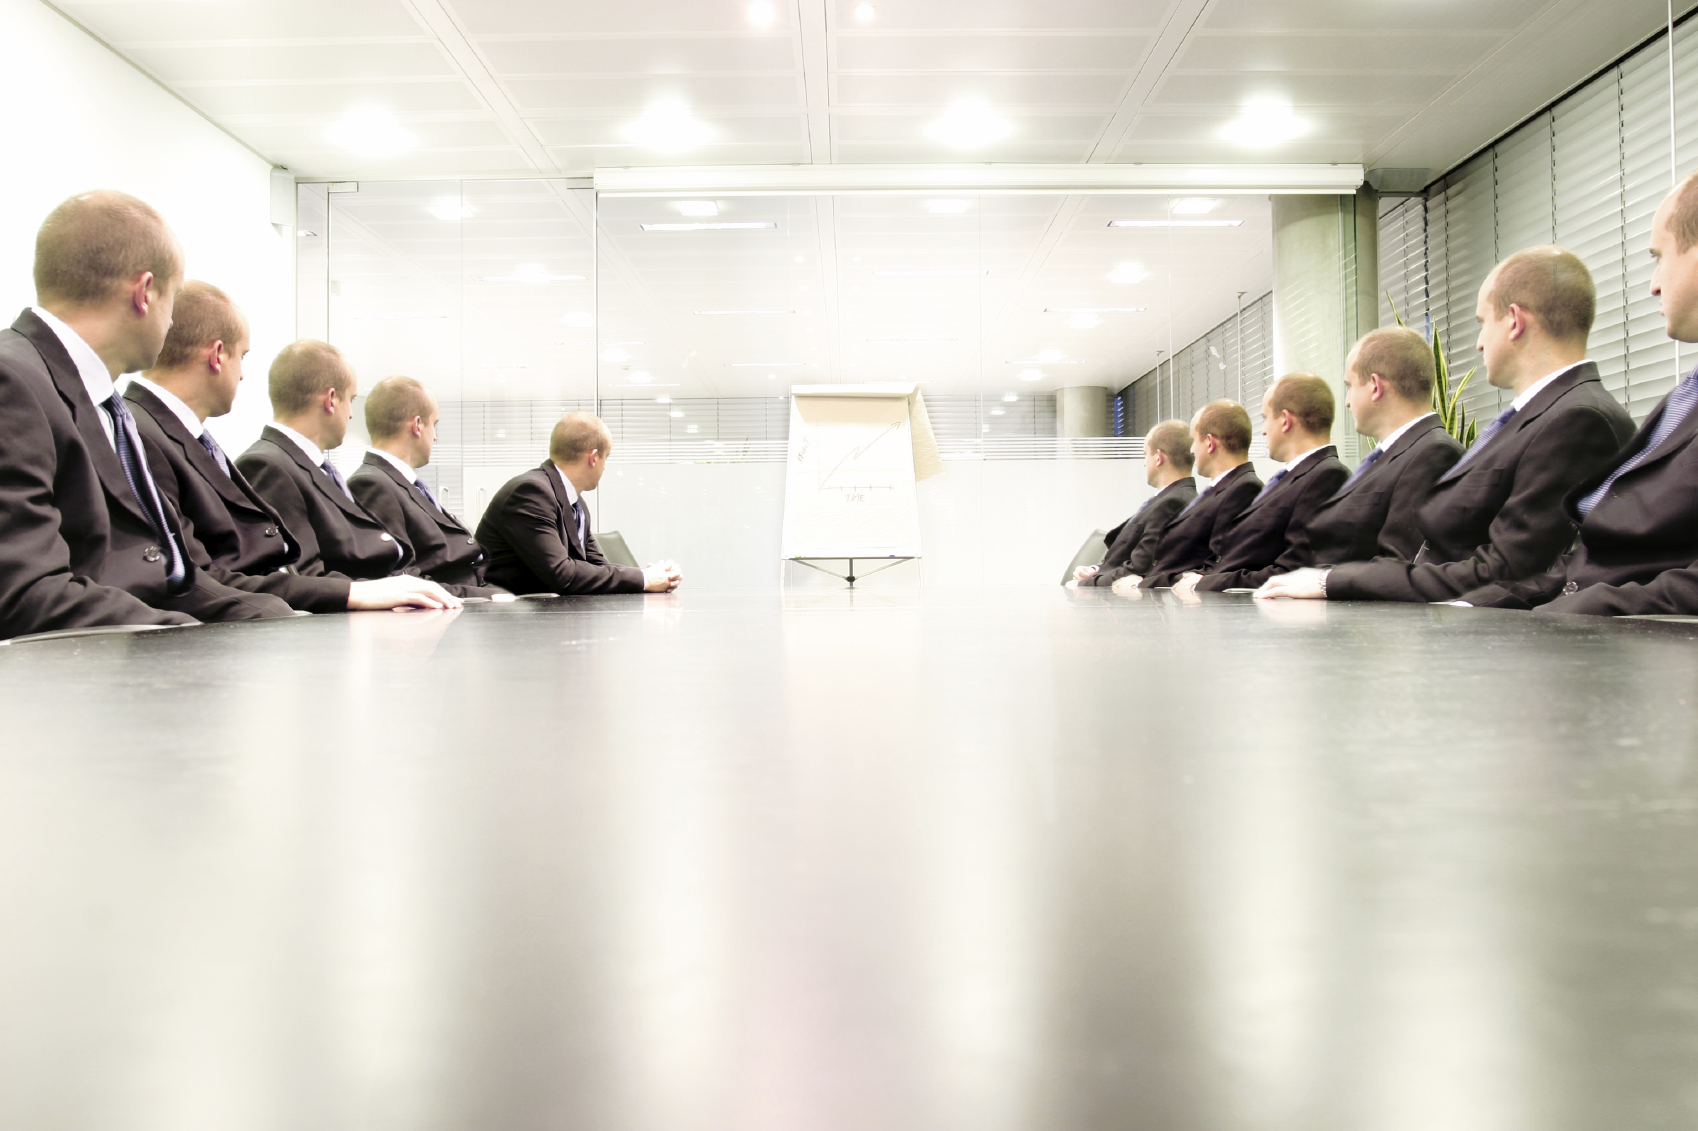
\includegraphics[width=0.9\textwidth]{praesentation_stress.jpg} 
	\end{center}
\end{frame}

\begin{frame}
	\frametitle{Code-Rosinen}
	
	\begin{itemize}
		\item Dispatcher-Funktion
		\item Callbacks und Handles
	\end{itemize}
\end{frame}

\end{document}
